\documentclass[12pt]{article}
\usepackage[utf8]{inputenc}
\usepackage{amssymb,amsmath}
\usepackage{hyperref}
\usepackage{graphicx}
\usepackage{color}
\definecolor{gray}{gray}{.75}
\author{Claas Jaehrling, Sven-Hendrik Haase}
\title{RS1 HA zum 16.12.11}
\date{\today}
\begin{document}
\setcounter{secnumdepth}{0}
\maketitle

\section{Aufgabe 9.1}
\subsection{(a)}
Der Hauptautomat zählt die Zustände Z0, Z1, Z2, Z6, Z7,
Z8, Z9, Z0,... weiter, während ein trivialer Automat dazwischen eine
Zählvariable hochzählt. \\
Zusätzlich wird noch eine Variable t für den Taster benötigt, die
erfasst, wann eine Fußgänger-Grünphase eingeleitet wird. \\
Das System ähnelt damit dem Kontrollfluss in Java:
t wird auf 0 gesetzt. \\
Danach schaltet der Hauptautomat einen Zustand in einer
Endlosschleife weiter, dabei wird die Zählmethode des Zählers
aufgerufen und der aktuelle Zustand als Parameter übergeben.\\
Hier wird eine im Sekundentakt zählende for-Schleife durchwandert,
welche als Abbruchbedingung hat, dass die Zählvariable eine
bestimmte Größe erreicht hat: \\
einige Sekunden für Z1, Z2, Z7 und Z8 sowie für Z0 bei t = 1  \\
bzw. 30 Sekunden für Z6 und Z9.
Danach wird die Zählvariable auf 0 resettet und der Kontrollfluss
geht zurück an den Hauptautomaten.

Demnach gehen von allen durchlaufenen Zuständen und vom Taster t
Leitungen zum Zählautomaten und auch immer zum folgenden
durchlaufbaren Zustand zurück.
\subsection{(b)}
Dies ist bei meiner Interpretation des Automatensystems relativ egal,
allerdings ist mein Zählautomat nicht allzu trivial...
\subsection{(c)}


\section{Aufgabe 9.2}
\subsection{(a)}
Übergangs- und Ausgangstabellen: \\
\begin{tabular} {rlll|ll}
z1 & z0 & x1 & x0 & z1+ & z0+ \\ \hline 
0 & 0 & 0 & 0 & 0 & 1\\
0 & 0 & 0 & 1 & 0 & 0\\
0 & 0 & 1 & 0 & 0 & 1\\
0 & 0 & 1 & 1 & 0 & 0\\
0 & 1 & 0 & 0 & 0 & 1\\
0 & 1 & 0 & 1 & 1 & 0\\
0 & 1 & 1 & 0 & 0 & 1\\
0 & 1 & 1 & 1 & 1 & 1\\
1 & 0 & 0 & 0 & 1 & 0\\
1 & 0 & 0 & 1 & 1 & 0\\
1 & 0 & 1 & 0 & 0 & 1\\
1 & 0 & 1 & 1 & 0 & 0\\
1 & 1 & 0 & 0 & 1 & 0\\
1 & 1 & 0 & 1 & 1 & 1\\
1 & 1 & 1 & 0 & 1 & 0\\
1 & 1 & 1 & 1 & 0 & 1
\end{tabular}
\subsection{(b)}
\subsection{(c)}

\section{Aufgabe 9.3}
\begin{align}
y = \overline{(a \land b) \lor ((c \lor d) \land (e \lor f))}
\end{align}
\subsection{(a)}
Ein solches Komplexgatter könnte man als eine Kombination aus einem
AND-Gatter (a AND b), zwei OR-Gattern (c OR d bzw. e OR f), noch
einem AND-Gatter ((c OR d) AND (e OR f)) sowie einem NOR-Gatter
darstellen.
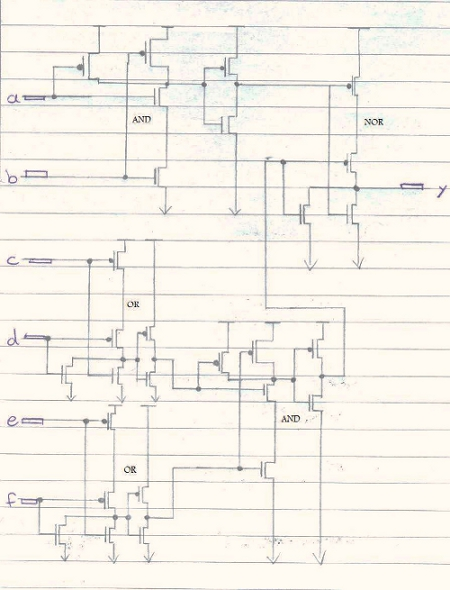
\includegraphics{Schaltskizze93a}
subsection{(b)}
Dieses Komplexgatter benötigt 28 Transistoren, eine herkömmliche CMOS-Gatter-Realisierung dagegen nur 12.

\section{Aufgabe 9.4}
siehe Anhang

\end{document}
